% !TeX root = ../../thesis.tex

\section{\acs{UEFI} Shell}

Part of the family of \ac{UEFI} specifications is a shell specification which defines a feature rich \ac{UEFI} shell application to interact with the \ac{UEFI} environment \cite[Section 1.1]{uefi-shell-spec}.
It offers commands relating to boot and general configuration, device and driver management, file system access, networking \cite[Section 5.1]{uefi-shell-spec} and scripting \cite[Section 4]{uefi-shell-spec}.
The \ac{UEFI} shell may already be part of the boot options but can always be supplied on removable media in the default boot path.
During initialization the shell produces default mappings for file systems and block devices, this defines names that can be used interchangably with their device paths when issuing shell commands \cite[Section 3.7.2]{uefi-shell-spec}.
These mappings are designed to be consistent across reboots as long as the hardware configuration stays the same, they are comparable to Windows partition letters \cite[Appendix A]{uefi-shell-spec}.
It also produces the initial output of what is equivalent to the invocation of the commands \program{ver} and \program{map} \cite[Section 3.3]{uefi-shell-spec}.
\program{ver} displays the version of the \ac{UEFI} specification the firmware conforms to, while map shows the current device mapping \cite[Section 5.3]{uefi-shell-spec}.
\autoref{fig:uefi-shell} depicts an exemplary output of the \ac{EDK} II \ac{UEFI} shell.

The \ac{UEFI} shell is a great tool to visualize the \ac{UEFI} environment.
With the \program{devtree} command we can see all handles of devices complying with the \ac{UEFI} driver model.
It is also a great reference to understand device paths.


When we inspect the mapping table we can see \lstinline{FSx:} and \lstinline{BLKx:} aliases, \lstinline{FSx:} maps to file systems and \lstinline{BLKx:} to block devices.
This identification is performed via instances of the \hyperref[lst:simple-file-system-protocol]{Simple File System Protocol} and \TODO{double check} Block \ac{I/O} Protocol.
% explain Simple File System Protocol
The \hyperref[lst:simple-file-system-protocol]{Simple File System Protocol} \cite[Section 13.4]{uefi-spec} provides, together with the \hyperref[lst:simple-file-system-protocol]{File Protocol}, file-type access to the device it is installed on \cite[Section 13.5]{uefi-spec}.
The two protocols are independent of the underlying file system the media is formatted with.



\TODO{me}

\begin{figure}[htb]
    \centering
    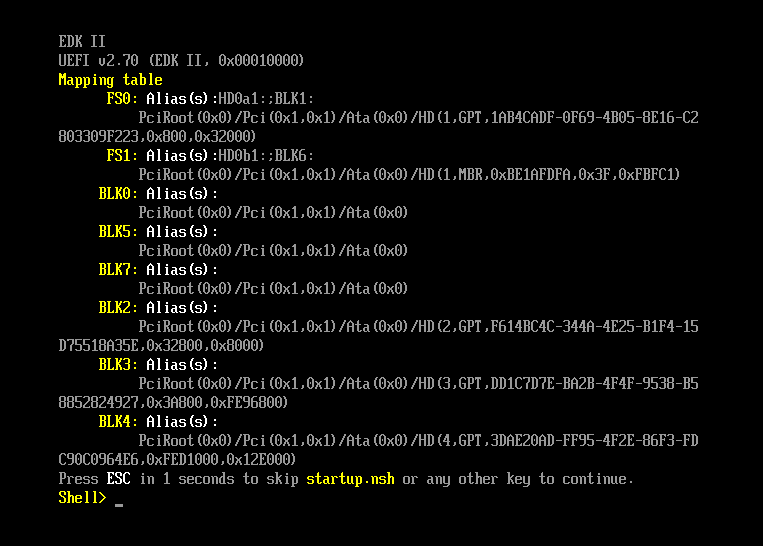
\includegraphics[width=1.0\textwidth]{uefi_shell.png}
    \caption{\ac{UEFI} command prompt}
    \label{fig:uefi-shell}
\end{figure}
